%% The following is a directive for TeXShop to indicate the main file
%%!TEX root = ../diss.tex

\chapter{Oxygen enhanced MRI - Validation of method in animals}
\label{ch:oemri}

\section{Preface}

Stuff about contributions 
% ======================================================================
\section{Introduction}
% ======================================================================

Dynamic oxygen enhanced MRI (dOE-MRI) has recently been proposed by our group to assess tumour oxygenation in vivo using MRI~\cite{Moosvi:2018ca}. 
This technique measures T1-weighted changes in tissues in response to a cycling oxygen challenge, with the responsive signals detected using independent component analysis (ICA). 
Briefly, oxygenation can be assessed \emph{in vivo} by administering a simple gas challenge (switching between two-minute periods of medical air and 100\% O$_2$) during the dOE-MRI scan and then using ICA to extract the tissue response.
ICA is a blind-source separation algorithm that separates multiple signal sources by maximizing statistical independence of individual components~\cite{Hyvarinen:2000vk}.
Various flavours of oxygen-enhanced MRI (OE-MRI) have been proposed but all essentially leverage the paramagnetic properties of inhaled oxygen.
White et al. has shown that OE-MRI may be very relevant in developing prognostic factors to predict tumour response to hypofractionation by stratifying tumours that may benefit from oxygen breathing during irradiation~\cite{White:2016fz}.
In this study, we apply dOE-MRI to mice bearing tumour xenografts to assess the effect of a common antiangiogenic agent.

Aberrant angiogenesis, poor blood perfusion, a chaotic vascular network all limit oxygen delivery to cells and contribute to formation of hypoxic regions in tumours.
The binding of vascular endothelial growth factors (VEGF) to the VEGF receptor is a key driver of angiogenesis.
Bevacizumab (Avastin) is a monoclonal antibody that binds VEGF extracellularly, preventing the interaction of of VEGF to its receptors and inhibits angiogenesis 
Avastin has been used clinically to treat breast, colon, colorectal, lung, brain, ovarian, cervical, and other cancers~\cite{AvastinIndications}\todo{cite Genentech}%https://www.gene.com/download/pdf/avastin_prescribing.pdf]. 
VEGF ablation has been shown to at least temporarily reduce vascular permeability and increase tumour oxygenation in some models~\cite{OConnor:2012iea}\todo{this review has lots of relevant refs, better to cite directly than a review}. 
We hypothesized that dOE-MRI with groupICA can detect VEGF ablation-induced changes to oxygenation of SCCVII tumours 48 hours following treatment.

% ======================================================================
\section{Derivation of lognormal perfusion}
% ======================================================================

% ======================================================================
\section{Methods}
% ======================================================================
\subsection{Animals}
Female NRG (NOD rag gamma) mice were implanted with murine squamous cell carcinoma (SCCVII; 5x10$^5$ cells in 50$\mu$l serum-free media; cells provided by Dr. J. Evans) in the dorsal subcutaneous region.
Approximately X \todo{how many days?} days later, tumours were imaged when their largest diameters reached approximately 8-10 mm.
All mice were injected with 60 mg/kg pimonidazole hydrochloride (HypoxyProbe) 30 min prior to imaging to label hypoxic cells and were euthanized within 15 min of imaging completion.
Mice were anesthetized with isoflurane using 1.5-2.0\% isoflurane for the duration of MR imaging sessions until euthanasia, and were positioned supine on the custom surface coil apparatus.
Throughout the imaging session, a small animal monitoring system (SAII Instruments, Stony Brook, NY, USA) was used to monitor respiration rate, varying between 80-100 breaths per minute, and body temperature, maintained at 36.8 $\pm$ 0.5$^\circ$C using a continuous airflow heater. 
tumours were embedded and frozen in optimum cutting temperature medium (OCT; Tissue-TEK).
All animal experimental procedures were carried out in compliance with the guidelines of the Canadian Council for Animal Care and were approved by the institutional Animal Care Committee.

\subsection{Immunohistochemistry}
Co-planar MRI slices and histological sections were obtained by imaging perpendicular to the longest tumour axis in MRI and serial-step 10 $\mu m$ cryosections were cut at 0.5-mm intervals in the same plane.
Slides were then fixed in acetone-methanol for 10 min and whole sections were immunohistochemically stained~\cite{Kalra:2017is} for CD31 (PECAM; visualized using secondaries labeled with Alexa 647nm) to label blood vessels, and for pimonidazole (HypoxyProbe-1; visualized using secondary labeled with Alexa 546nm) to label hypoxic cells. Sections were then stained using Hoechst 33342 (bisbenzimide) to label all cell nuclei.
Whole-tumour sections were imaged using a robotic fluorescence microscope (Zeiss Axioimager Z1), a cooled, monochrome CCD camera (Retiga 4000R; QImaging), a motorized slide loader and x-y stage (Ludl Electronic Products) and customized ImageJ software~\cite{Collins:2007jr}. 
Adjacent microscope fields of view were tiled such that images of entire tumour cryosections were captured at a resolution of 1.5 $\mu m$/pixel. 
Using anatomical landmarks and accumulated thicknesses of serial-step sections as estimates of distances from the edges of whole tumours, sections were chosen to match the MR slices. 
ImageJ and user-supplied algorithms were used to super impose digital images which were then manually cropped to tumour tissue boundaries with staining artifacts removed. 
A threshold was applied to images to identify positive pimonidazole staining, and the number of positive pixels was determined as a percentage of the total number of pixels in the tumour image. 
Overlaid greyscale images were converted to false colour for visualization with pimonidazole as green and CD31 as magenta~\todo{need to make sure final colours are consistent}.

\subsection{MR Imaging}
Imaging was performed using a 7T scanner (Bruker Biospec) with a transmit quadrature volume coil and a custom built surface receive coil. 
An axial RARE image was acquired to localize the tumour (TE/TR=10.7/4250ms, RARE factor 8) and a T$_1$ map was acquired using the Look-Locker method.
Dynamic oxygen enhanced MRI (dOE-MRI) scans were acquired with a 2D multi-slice FLASH-based sequence for a total scan time of about 14 minutes.
During the dOE-MRI scan, breathing gas was alternated between medical air and 100\% oxygen every 2 minutes using a 3-channel gas mixer (CWE, Philadelphia, USA) for a total of 3 air-oxygen-air cycles.
All scans were acquired with the same spatial resolution and geometry and an experienced operator outlined the tumour on each slice of the RARE image to construct the region of interest (ROI) for each animal and then transferred to all other scans.

\subsection{dOE-MRI Analysis}
A suite of in-house software was developed using the python machine learning library scikit-learn~\cite{Pedregosa:2011tv}, specifically \texttt{sklearn.decomposition.FastICA} based on the technique described by Hyvarinen~\cite{Hyvarinen:2000vk}.
The FastICA algorithm is applied to serially acquired T$_1$W images and the output is a paired set of components and weighting factors for each voxel in the dataset.
The deflation-based FastICA (python package scikit.sklearn v0.17.1) was used to analyze the data. 
Extracted independent components are not ordered and while the component selection can be automated, in this study an observer was assigned to select the appropriate component.
The number of independent components for each imaging session was chosen by the operator and ranged from 4-9 to ensure the cyclic behaviour of the T$_1$W signal intensity corresponding to the gas challenge appeared in only one component. 
The dOE-MRI maps were obtained by dividing the ICA weighting-factor maps by the mean signal-intensity maps to obtain a spatial map for the strength of a particular voxel's contribution to the component of interest.
In these dOE-MRI maps, voxels are coloured to indicate the amount by which a given pixel intensity time course is modulated by the oxygen-related component. 
Final normalized dOE-MRI maps were obtained by dividing each pixel of the component map for each animal with the mean signal-intensity over time of the corresponding pixel in the dOE-MRI scan. 
Mean values are reported as a marker for tumour oxygenation with high values indicating increased oxygenation while negative values suggest decreased oxygenation or increased levels of hypoxia. 
Mann-WhitneyU parametric t-tests are used to assess the difference between experimental groups and Hedge's g was calculated to determine effect size when the t-test was significant (p$<$0.05).
The green-white-purple colour spectrum depicts the degree to which voxels respond to the cycled gas challenge.
Purple indicates O$_2$-positive voxels whose time course exhibits a higher and more positive contribution from the corresponding ICA component, representing an increase in T$_1$W signal intensity in response to the supplied 100 \% oxygen, and corresponding to areas with excess dissolved oxygen. 
O$_2$-negative voxels that show a decrease in T$_1$W signal intensity with a negative contribution from the corresponding ICA component under 100 \% oxygen breathing are depicted as green. 
Regions whose T$_1$W signal intensity time courses responds only weakly or not at all to the gas challenge are shown in white hues.
A feature of FastICA is that the norm of each component is normalized to 1 ($||c_i||=1, \forall I$) and the corresponding weighting factor map carries the scaling factor.
To compare dOE-MRI maps between mice with different temporal resolutions, a scaling factor was applied (see section~\ref{res1} and the Appendix).

% ======================================================================
\section{Results}
% ======================================================================

%%%%%%%%%%%%%%%%% ############ BEGIN section from paper 1 ############ 

\subsection{ICA enabled dOE-MRI detects variable oxygenation in a range of tumour models}
tumours of human and murine origin and comprising a variety of tumour microenvironments were imaged, including fast growing, highly vascularized murine squamous cell (SCCVII) and human ovarian carcinomas (SKOV3), slower growing and well vascularized human breast cancer (BT-474), as well as a relatively fast growing but more poorly vascularized human colon colorectal carcinoma (HCT-116).
The inter-model heterogeneity of the tumours is reflected in the mean fraction of negative voxels in the dOE-MRI maps, which were 46 $\pm$ 6\% for BT-474, 36$\pm$3\% for HCT-116, 31$\pm$5\% for SCCVII, and 14$\pm$4\% for SKOV3 tumours. 
Considerable intra-tumour heterogeneity is also observed within some models, particularly the BT474.
dOE-MRI maps representing the mean fraction of negative voxels are shown for each tumour type in Figure~\ref{versatile}.
\begin{figure}[htbp]
   \centering
   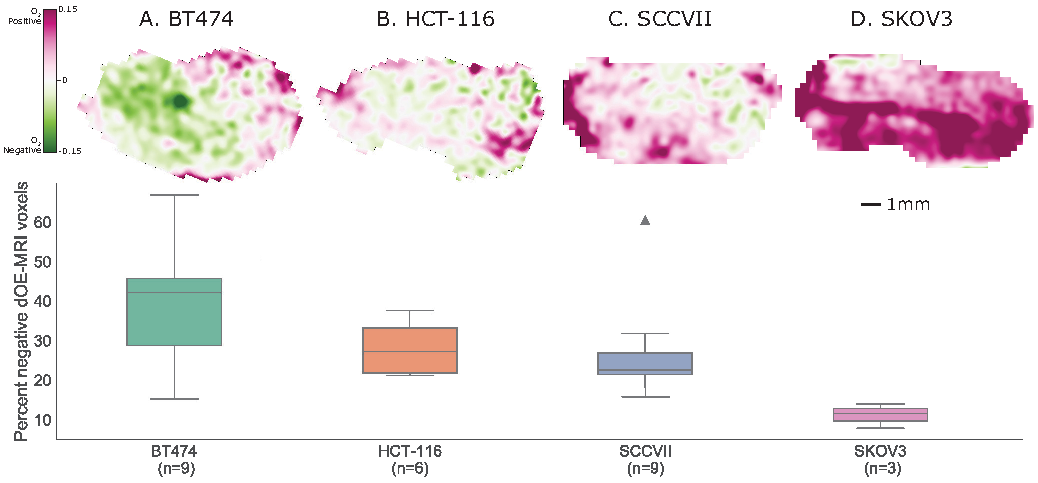
\includegraphics[width=\textwidth]{oemri_thesis1/oemri_thesis1-images/fig2_versatile.pdf} % requires the graphicx package
   \caption{Top: dOE-MRI maps for four tumour models HCT-116, BT-474, SCCVII, and SKOV3 are shown. Chosen slices are representative of the mean percent negative dOE-MRI fraction for the respective tumour model.
Bottom: The box-whisker plot shows the quartiles of percent negative dOE-MRI voxels for all imaged tumours.
\label{versatile}}
\end{figure}

\subsection{dOE-MRI maps correspond to matched histology sections}

tumour tissue cryosections obtained to match MR imaging slices were stained for vasculature (CD31) and regions of pimonidazole-labeled hypoxia and are compared side-by-side; Figures~\ref{fig_sccvii} and~\ref{fig_hct116} provide five examples for each of SCCVII and HCT-116 tumour models for detailed review.
Generally, in corresponding dOE-MRI maps for both tumour models O$_2$-positive voxels align with the most oxygenated regions of histology sections, where pimonidazole labeling is absent, however many areas of mismatch are also observed. 
More consistent is that O$_2$-positive voxels do not typically correspond to tissues identified as hypoxic in the histology sections (i.e. labeled with pimonidazole).
In general, the more necrotic HCT-116 tumours have fewer oxygenated (O$_2$-positive) regions and significantly more hypoxic (O$_2$-negative) regions in the dOE-MRI maps, compared to the SCCVII tumours that have no necrosis. 
Pimonidazole labeling is heterogeneously dispersed within regions of viable tissue containing tumour blood vessels for both SCCVII tumours, Figure~\ref{fig_sccvii}, and HCT-116 tumours, which typically have greater amounts of necrosis, Figure~\ref{fig_hct116}.
Figure~\ref{histo_correlations} shows the fraction of negative dOE-MRI voxels correlated with the histological hypoxic fraction. 
For SCCVII tumours (n=9) there was an excellent correlation, with Pearson's r = 0.91 (\textit{p}=0.0016). 
However the correlation in the HCT-116 tumours (n=6) was poor, with r=0.13 (\textit{p}=0.81). 

\begin{figure}[htbp]
   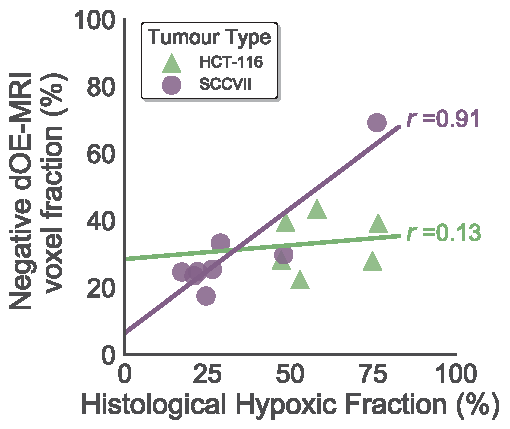
\includegraphics[width=\textwidth]{oemri_thesis1/oemri_thesis1-images/fig5_histocorrelation.pdf} % requires the graphicx package
   \caption{The proportion of negative dOE-MRI voxels is plotted against the histological hypoxic fractions with Pearson's r = 0.91 for SCCVII tumours and r = 0.13 for HCT-116 tumours.
   \label{histo_correlations}}
\end{figure}

\begin{figure}[htbp]
   \centering
   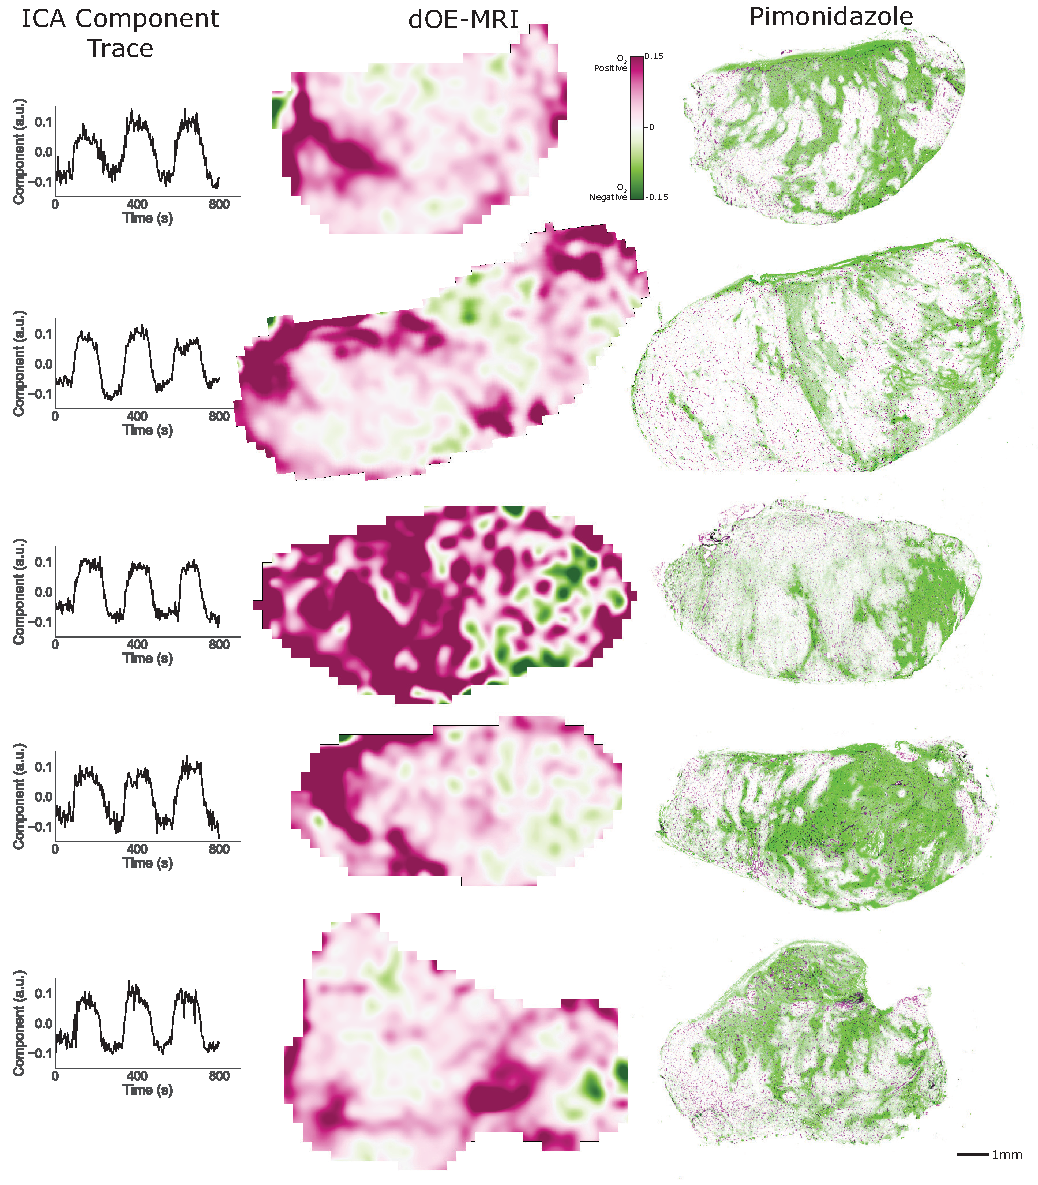
\includegraphics[width=0.9\textwidth]{oemri_thesis1/oemri_thesis1-images/fig6_sccvii.pdf} % requires the graphicx package
   \caption{SCCVII murine tumours with slice-matched histological images depicting pimonidazole-labeled hypoxia (green) and CD31-stained vasculature (purple) are shown next to the dOE-MRI parameter maps similarly colored with O$_2$-positive (purple) and O$_2$-negative (green) areas. Corresponding ICA extracted components are also shown.
   \label{fig_sccvii}}
\end{figure}
\begin{figure}[htbp]
   \centering
   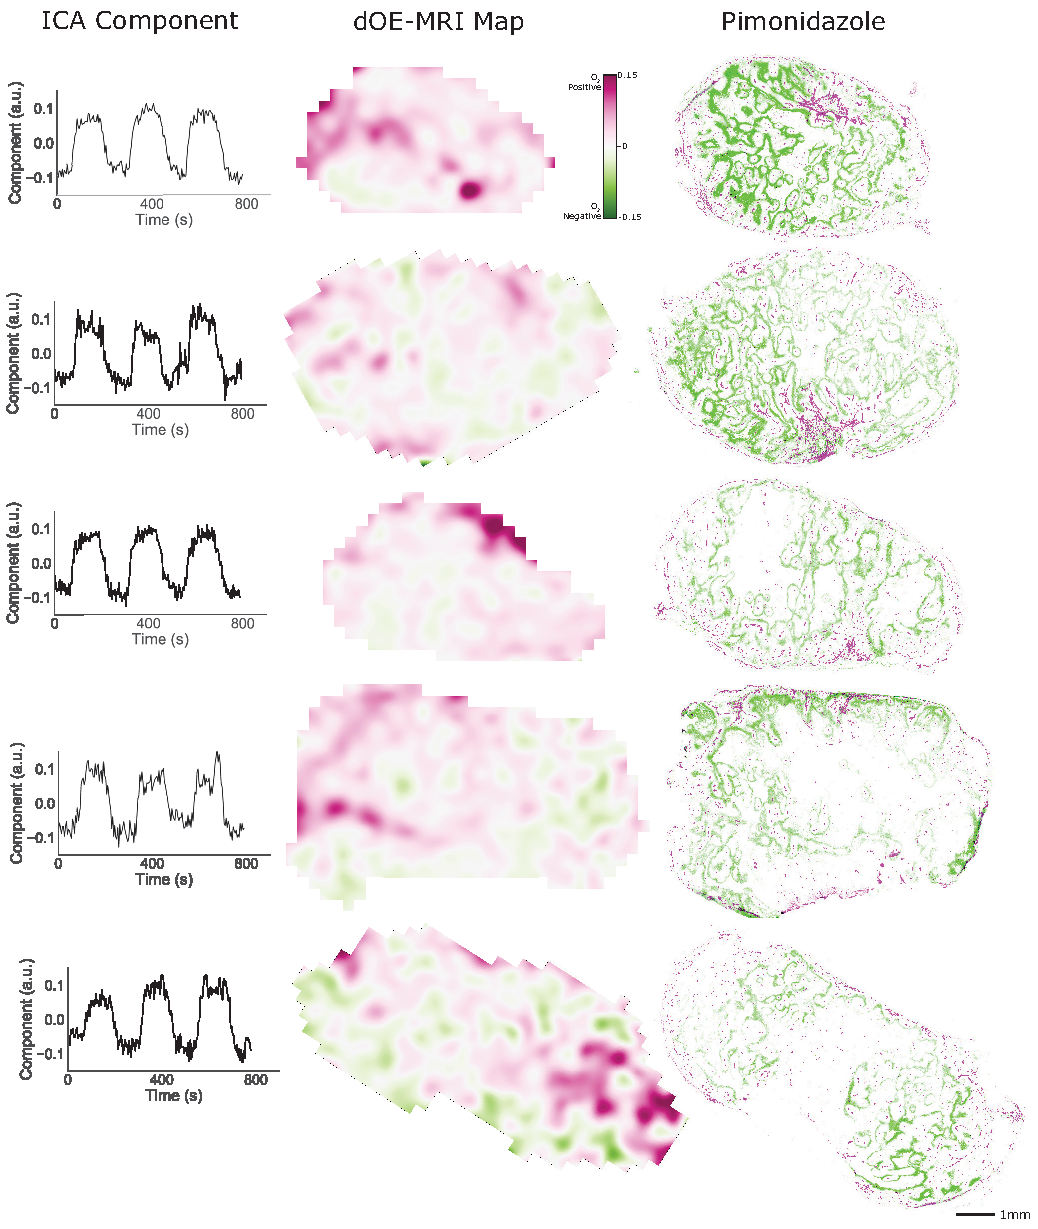
\includegraphics[width=0.9\textwidth]{oemri_thesis1/oemri_thesis1-images/fig7_hct116.pdf} % requires the graphicx package
   \caption{HCT-116 human colorectal xenografts with slice-matched histological images depicting pimonidazole-labeled hypoxia (green) and CD31-stained vasculature (purple) are shown next to the dOE-MRI parameter maps similarly colored with O$_2$-positive (purple) and O$_2$-negative (green) areas. Corresponding ICA extracted components are also shown.
   \label{fig_hct116}}
\end{figure}

%%%%%%%%%%%%%%%%% ############ END section from paper 1########### 

%%%%%%%%%%%%%%%%% ############ BEGIN section about fitting ############ 
\subsection{Fitting the cycling component with the lognormal replenishment model}

Lorem ipsum dolor sit amet, consectetur adipiscing elit. Etiam ullamcorper pretium neque, elementum pulvinar justo. Pellentesque aliquet, enim nec pulvinar scelerisque, erat risus convallis nibh, eget finibus diam massa ut diam. Sed eget dictum ex, at pellentesque sem. Mauris quis tincidunt turpis. Vestibulum ultrices lorem quis ex accumsan finibus. Sed mollis erat vitae magna fermentum pulvinar. Mauris orci odio, ullamcorper vitae eros porta, blandit ornare orci. Suspendisse potenti. 

Mauris ultrices, nibh in rutrum eleifend, nisl sapien suscipit ipsum, finibus imperdiet metus tellus in nunc. Fusce eget tellus tincidunt lectus convallis elementum quis sed ante. Nullam nisl tellus, gravida nec arcu nec, bibendum finibus ipsum. Proin eu turpis quam. Sed faucibus, urna id consequat placerat, enim ligula porttitor velit, id congue eros elit a eros. Sed pharetra nunc rutrum massa auctor iaculis. Interdum et malesuada fames ac ante ipsum primis in faucibus. Nunc quis sapien lacus. Morbi suscipit sed ante id.

\begin{figure}[htbp]
   \centering
   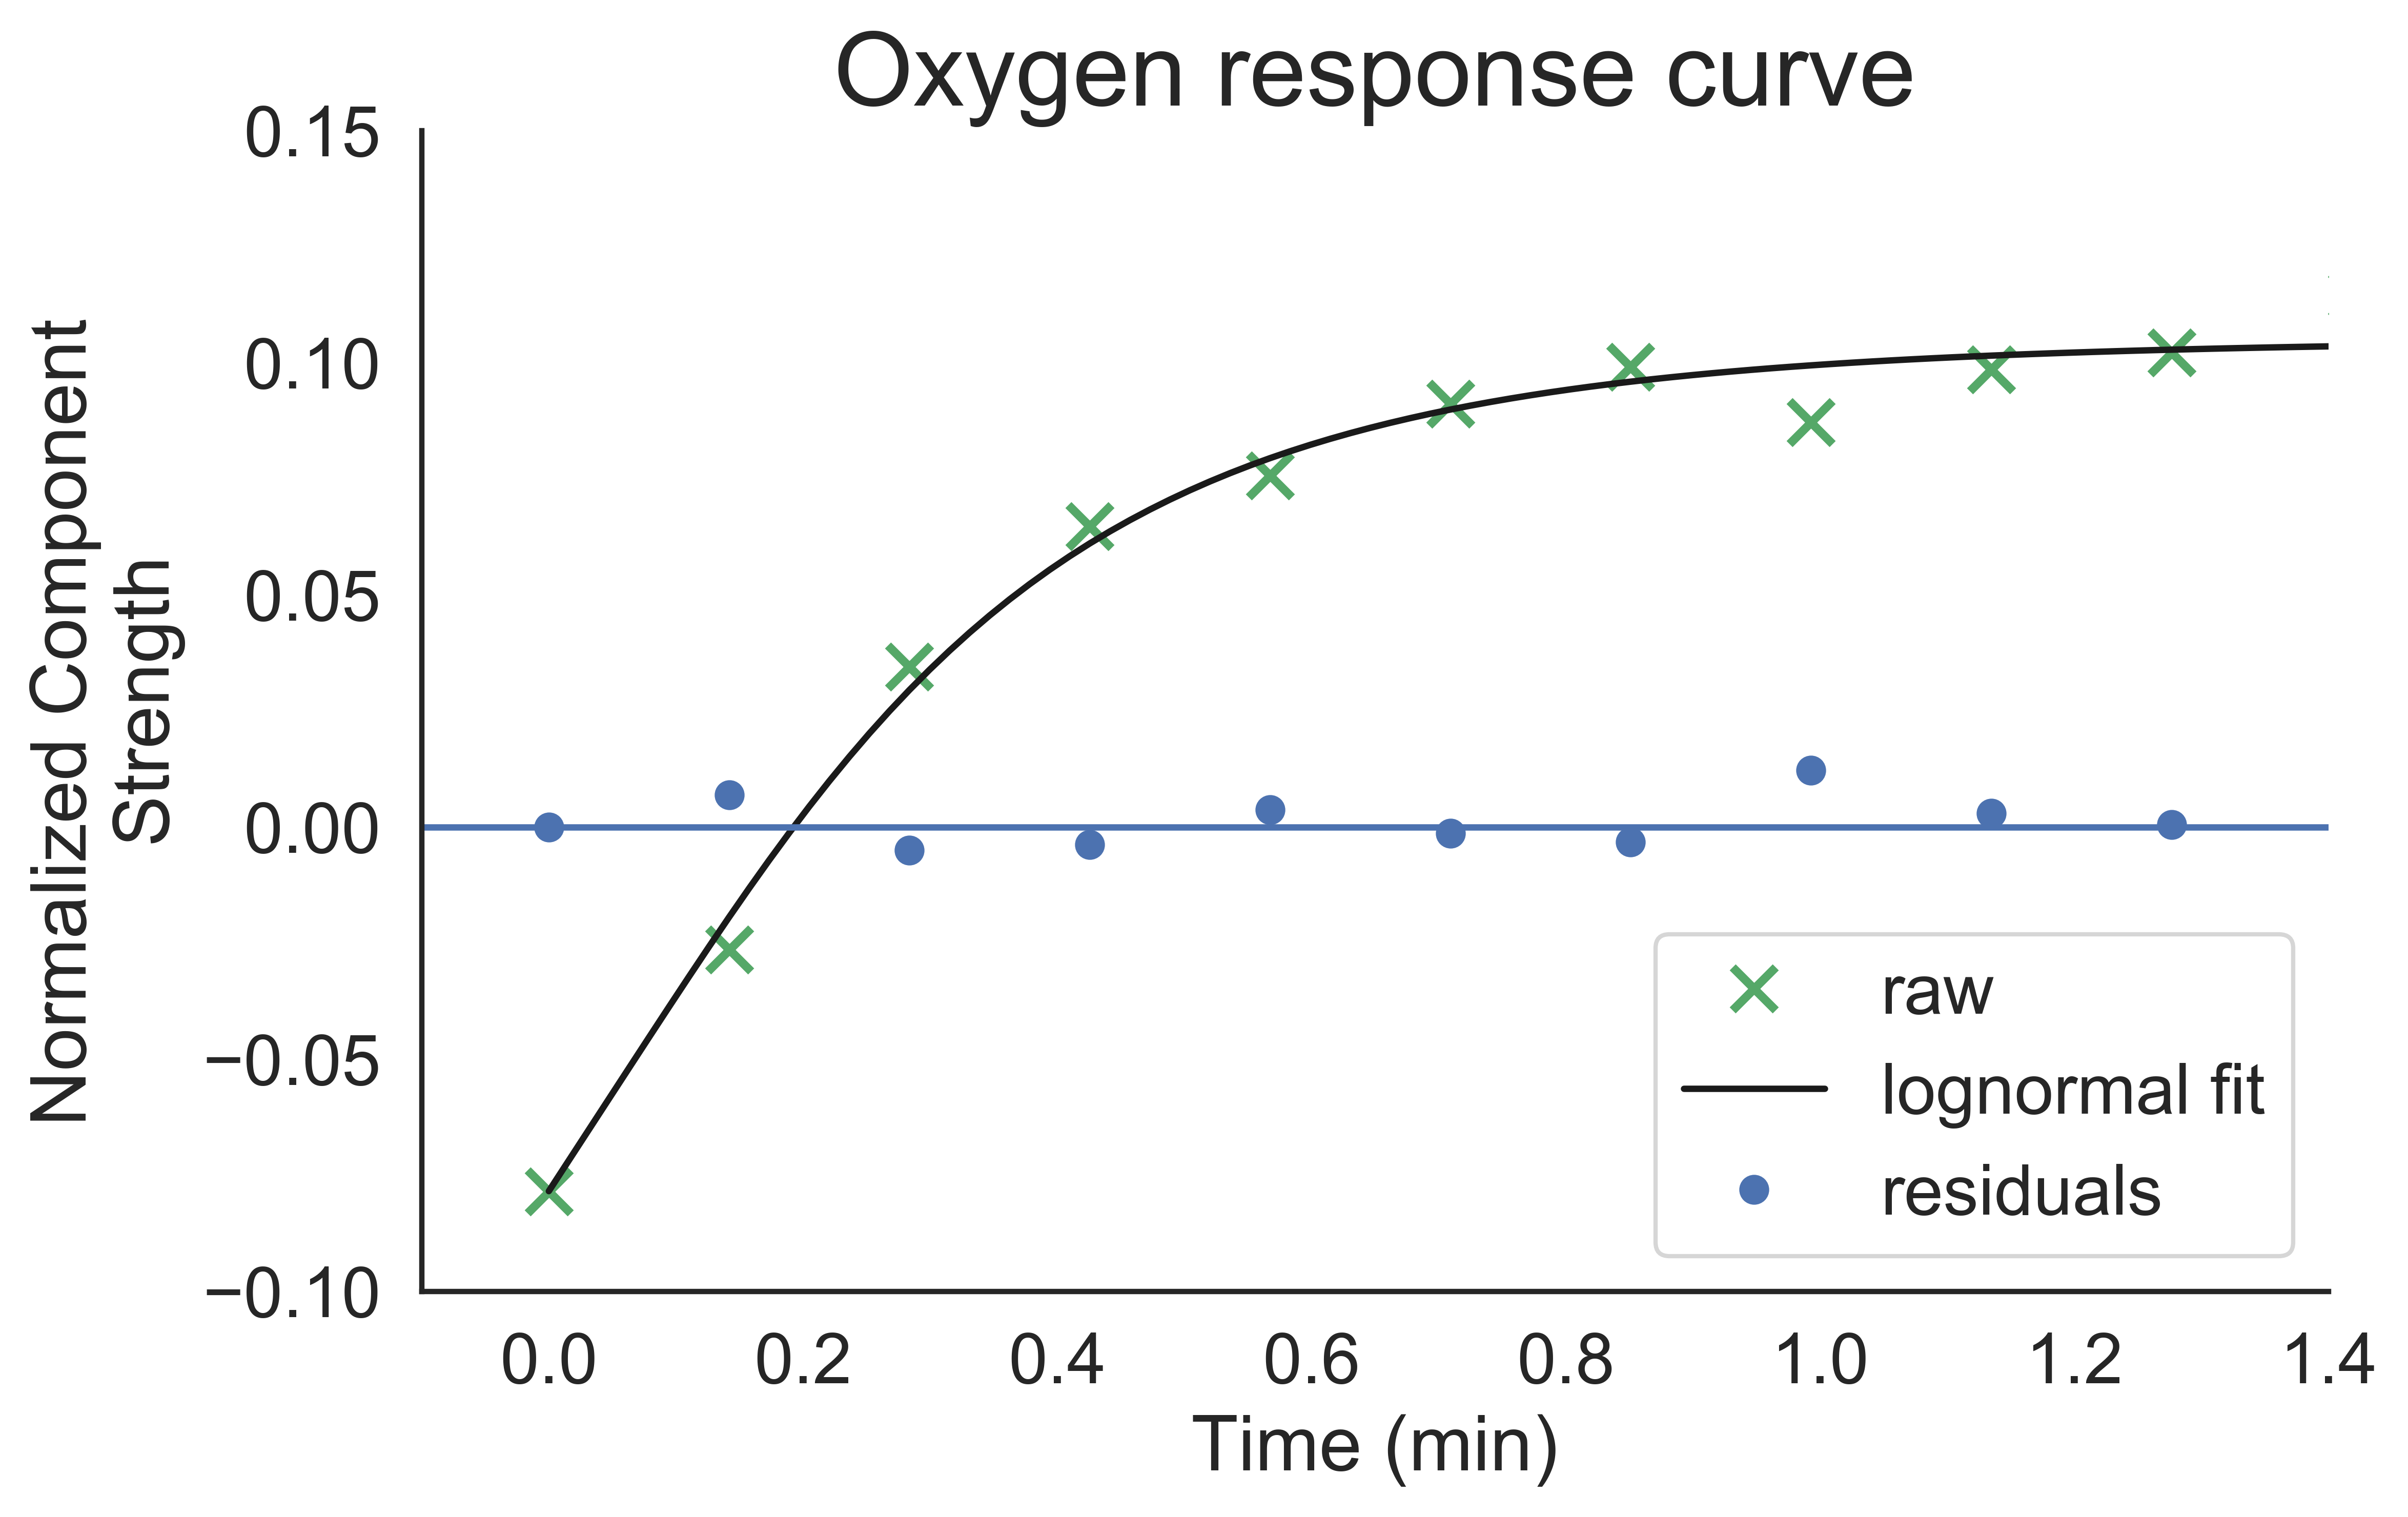
\includegraphics[width=0.5\textwidth]{oemri_thesis2/oemri_thesis2-images/technical_SampleFit.png} % requires the graphicx package
   \caption{}
   \label{subSample}
\end{figure}

\begin{figure}[htbp]
   \centering
   \includegraphics[width=\textwidth]{oemri_thesis2/oemri_thesis2-images/technical_dOE-MRIfits.pdf} % requires the graphicx package
   \caption{}
   \label{subSample}
\end{figure}

%%%%%%%%%%%%%%%%% ############ END section about fitting ############ 

% ======================================================================
\section{Discussion}
% ======================================================================

A limitation of OE-MRI is the difficulty in interpreting areas that do not show a reduction in T$_1$ as they may be either dead tissues that are \textit{unperfused and not oxygenated} or living, viable tissues that are \textit{perfused but not oxygenated} due to poor oxygen content of the supplying vessels. 
The latter population are of greater interest to the oncology community as it is these hypoxic but viable cells that have significant influence on treatment outcomes~\cite{Horsman:2016go}. 
The dOE-MRI technique presented here successfully correlates tumour oxygenation dOE-MRI and histology measures in SCCVII tumours but, despite improvements to sensitivity, a similar quantitative comparison in the HCT-116 tumour line showed poorer association (Fig.~\ref{histo_correlations}). 
This is likely attributable to the much higher amounts of necrosis typical of the HCT-116 model relative to SCCVII (Figs.~\ref{fig_sccvii} and \ref{fig_hct116}).
Mitigations to this limitation have been explored elsewhere and generally require a perfusion mask or $T_2^*$ - either technique can be added to the OE-MRI method proposed here to exclude necrosis and further improve sensitivity of the technique.

Application of existing OE-MRI techniques across a range of tumour models with varying perfusion characteristics has yielded mixed success without masking for perfused tissue.
For instance, O'Connor reported that in the highly perfused 786-0-R tumour lines, 85-96\% of all imaged tumour voxels were deemed to be oxygen-enhancing~\cite{OConnor:2016ee}.
In those tumours, there was a good correlation between histological hypoxic fraction and oxygen refractory voxels.
However, in the more weakly perfused SW620 tumours where only 76\% of the voxels are oxygen-enhancing, there were no significant correlations with the histological hypoxic fraction.
These issues were resolved by combining OE-MRI with DCE-MRI as a perfusion mask to select only perfused voxels for oxygenation assessment, thereby distinguishing between the viable hypoxic environment and necrotic dead tissues and improving the specificity and sensitivity of OE-MRI data. Using an IAUGC$_{60}$ map from DCE-MRI as a mask to obtain Oxy-R fractions O'Connor et al. showed good correlation with the histological hypoxic fraction~\cite{OConnor:2016ee}.
In more recent work, Little et al. showed oxygen enhancement in tumours with a histological hypoxic fraction as high as 43\%~\cite{Little:2018iu} and this translated very well to a study of six renal cell carcinoma patients.
Linnik et al. reported excellent correlation between percentage of ``negative AUC$_{OE}$'' ($O_2$-negative) voxels and percentage of hypoxic areas in the highly vascular preclinical U87MG tumour xenografts~\cite{Linnik:2013hf}.
A second approach for differentiating between viable but hypoxic regions and unperfused dead tissues, is to combine OE-MRI with $T_2^*$W acquisition and the BOLD effect to classify regions~\cite{Little:2018iu,Zhao:2015ez,White:2016fz,Burrell:2013je,Yang:2018vo} that show both effects. 
Excess oxygen in the blood will induce changes in Hb saturation, which alter the T2* resulting in a robust measure of areas with functioning vasculature. 
Conceivably, the saved acquisition time achieved with under-sampling T$_1$W dOE-MRI suggests that $T_2^*$W images could also be acquired to concurrently assess the blood oxygen level dependent (BOLD) response. 

Within the relatively short 14-minute imaging time, both the HCT-116 and SCCVII tumours show only minor changes in the oxygenation maps between cycles (Figure~\ref{fig_correlation}).
In longer imaging sessions, or during administration of an intervention, these same tumours may exhibit varying oxygenation patterns between cycles.
Periods of oxygen-starvation and re-oxygenation in tumours have been termed intermittent hypoxia and can arise due to temporary vessel occlusions~\cite{Dewhirst:2009de,Bayer:2011js}.
Recent work on measuring intermittent hypoxia in patients using R$_2^*$~\cite{Panek:2017ge} shows that interest in this phenomenon continues but the importance of intermittent hypoxia in tumours is unclear largely due to poor availability of techniques to measure it in the clinic~\cite{Michiels:2016hv}.
The relatively short imaging time for dOE-MRI makes assessing temporal oxygenation changes possible within a timescale on the order of minutes by comparing correlation maps generated from sequential cycles.

Typically, histological validation of MR data is done by collapsing rich histology data into a single metric, such as a hypoxic fraction, with whole-tumour or single-slice average comparisons.
While this is sometimes a useful validation approach, it may not reflect the highly heterogeneous patterns of hypoxia that are known to vary spatially and temporally, even within the same tumour, as well as between tumour types as highlighted in Figures~\ref{histo_correlations}-\ref{fig_hct116}. 
Further complications are encountered with respect to validation of tools to assess hypoxia considering that hypoxia is not simply a binary metric. Instead, tumour oxygenation exists as a spectrum beginning with some tissues that may be normoxic, at levels similar to neighbouring normal tissues of origin, and can continue decreasing through levels of hypoxia to near anoxia where cells are still viable but are no longer able to proliferate.
Eventually cells die in the absence of oxygen, and when this occurs in large numbers there can be significant regions of necrosis in solid tumours. 
A range of oxygenation levels are likely to be present in the highly heterogeneous microenvironments of all solid tumours, but what is of interest to the oncology community is \emph{clinically relevant} hypoxia~\cite{Horsman:2012kw}.
This refers to measurable tumour oxygenation levels that are biomarkers of physiologically meaningful phenomena, including patient prognosis or tumour sensitivity to treatments, such as immunotherapy or radiotherapy. The relevant oxygenation status for any biomarker of interest may include levels spanning from moderate to severely hypoxic. 
Pimonidazole has been demonstrated as a clinically relevant marker of hypoxia, but poor or inconsistent correlation with pimonidazole, as we have seen in our imaged tumours, does not exclude other measures of tumour oxygenation from potential utility.

Measurable pimonidazole-adduct formation occurs when the O$_2$ tension in the vicinity drops below 10 mmHg~\cite{Gross:1995wq} but in dOE-MRI, O$_2$-positive voxels are extracted as excess oxygen dissolves in the plasma and interstitial tissue fluid to decrease T$_1$.
Voxels where T$_1$ has significantly increased has previously been correlated to poorly perfused regions and likely corresponds to hypoxic regions where the excess oxygen is picked up by deoxyhemoglobin molecules~\cite{Linnik:2013hf,Burrell:2013je,Remmele:2012df}.
The exact mechanism for a T$_1$ increase as a result of oxygen inhalation has not yet been confirmed~\cite{Zhao:2015ez,Linnik:2013hf}, however, based on careful work of Silvennonin et al., characterizing behavior of T$_1$ in fresh bovine blood~\cite{Silvennoinen:2003gn}, we speculate the corresponding T$_1$W signal decrease may arise due to the conversion of deoxyhemoglobin to hemoglobin in the perfused vessels of hypoxic regions .
O$_2$-positive regions in dOE-MRI maps are generally in good agreement with well perfused areas of histology images for both HCT-116 and SCCVII tumours, as shown in Figures~\ref{fig_sccvii} and~\ref{fig_hct116}.
Voxels exhibiting signal reduction with the O$_2$ stimulus in dOE-MRI maps (O$_2$-negative, green) typically correspond with histology (pimonidazole, green) but not all pimonidazole-labeled regions appear as O$_2$-negative voxels.
Similarly, CD31-stained tumour regions are not exclusively O$_2$-positive in the dOE-MRI maps because not all tumour vessels are perfused.
In fact many perfused blood vessels are only intermittently perfused and consequently, the measurement of hypoxia is time-sensitive.
Mismatches between dOE-MRI and histology may be attributed in part to the different sensitivities and detection thresholds for measuring hypoxia and oxygenation in the dOE-MRI and histology-based modalities, as well as potential mismatch between the timing of pimonidazole-labeling and dOE-MRI data acquisition . 

\subsection{random snippets}
O$_2$ positive or O$_2$-negative fractions are immune to this phenomenon, information about the level of response can be retained simply by applying the scaling factor when comparing scans at different temporal resolutions
% ======================================================================
\section{Conclusions}
% ======================================================================
Hello

% ======================================================================
\section{Acknowledgments}
% ======================================================================

This work was supported by NSERC and CIHR.

% ======================================================================
 %\section{References}
% ======================================================================
%\bibliography{oemri2}

%\bibliographystyle{vancouver-authoryear}

%\end{document}